\input{../preambule.tex} 

% Modification des variables de session 
\input{../../variables.tex} 

\newcommand{\exercice}{2}
\makeindex
% custom footers and headers
\usepackage{fancyhdr}
\pagestyle{fancy}
\lhead{\nomcours}
\chead{}
\rhead{\cours}
\lfoot{ Exercice \exercice}
\cfoot{}
\rfoot{Page \thepage}
\renewcommand{\headrulewidth}{1pt}
\renewcommand{\footrulewidth}{1pt}
%
% my own titles

\makeatletter
\renewcommand{\maketitle}{
	\begin{center}
		\vspace{2ex}
		{\huge \textsc{\@title}}
		\vspace{1ex}
		\\
		\linia\\
		\@author \hfill \@date
		
		\linia\\
		\vspace{2ex}
	\end{center}
}



\makeatother
%%%
%%%----------%%%----------%%%----------%%%----------%%%

\begin{document}
	
	\title{Exercice \textnumero{}\exercice \\
		\\Mise en place d'un environnement de développement \\
		\SELinux
		
	}
	\author{\prof, \Cegep}
	\date{\session}
	
	\maketitle
	
	\begin{flushleft}
		\noindent \textbf{Évaluation :} formative \\
		\textbf {Travail de préférence individuel.}\\
		\textbf{Durée :} 2 heures \\
		\textbf{Système d'exploitation :} \SELinux \\
		\textbf{Environnement de virtualisation :} \Esx\\
		\textbf{Site de référence :}\url{https://doc.ubuntu-fr.org/ide}
		
	\end{flushleft}
	\rule{17cm}{0.1pt}
	
	
	\section{Définition}
	\begin{quotation}
		Un environnement de développement est un ensemble d'outils qui permet d'augmenter la productivité des programmeurs qui développent des logiciels. Il comporte un éditeur de texte destiné à la programmation, des fonctions qui permettent, par pression sur un bouton, de démarrer le compilateur ou l'éditeur de liens ainsi qu'un débogueur en ligne, qui permet d'exécuter ligne par ligne le programme en cours de construction[...]
		
		Dans un environnement de développement « intégré »[...]les outils sont prévus pour être utilisés ensemble. Les outils peuvent être intégrés dès le départ, c'est-à-dire qu'ils sont construits dans le but d'être utilisés ensemble. \cite{Wikipedia_EDI_2020}
	\end{quotation}
	
	\section{Prérequis VMware tools}
	
	Utiliser la page suivante pour vérifier ou installer VMware tools on Ubuntu 20.04 :
	\url{https://linuxconfig.org/install-vmware-tools-on-ubuntu-20-04-focal-fossa-linux}
	
	\section{On a besoin de quoi au juste ?}
	
	Nous allons construite un environnement avec deux IDE : 
	\begin{enumerate}[label=\arabic*)]
		\item \textbf{Eclipse} qui est un très bon IDE écrit en Java, extensible par des greffons, multi-langages et multi-plates-formes, qui s'intègre particulièrement bien à GNOME. \\
		Il permet de développé dans les langages : \textbf{Java, C, C++, Web, PHP, Python, Ruby .}
		
		\item\textbf{Visual Studio Code} un éditeur de code multi-plateforme, open source et gratuit, supportant une dizaine de langages.
		Il permet de développé dans les langages : \textbf{C\#, C/C++, Python, Go, PHP, Web, …}
		\vspace{10pt}
		
		
		
		Mais avant nous allons préparer nos environnements avec des outils complémentaires :
		
		\item \textbf{Git} : logiciel de gestion de versions décentralisée. 
		\item \textbf{Machine virtuelle Java} : Qui est un appareil informatique fictif qui exécute des programmes compilés sous forme de bytecode Java
		\item \textbf{.Net Core} : .NET Core est un cadriciel (Framework) Libre et Open Source pour les systèmes d'exploitation Windows, macOS et Linux. Il comprend CoreCLR, un environnement d'exécution complet de CLR, la machine virtuelle qui gère l'exécution des programmes .NET. 
		\item \textbf{Nginx} : Serveur Web.
		\item \textbf{MySQL} : Serveur de Base de données relationnel.
	\end{enumerate} 
	Voilà, vous aurez une machine virtuelle qui vous permettra de développer dans plusieurs langage.\\
	

\section{Espace disque}
Mais avant d'allez plus loin, vérifier l'espace disque utilisé avant les installations.
\index{df}\index{grep}
\begin{lstlisting}[language=bash]   ]
$df -h |grep /dev/sda > Bureau/espaceDiskAvantInstallation.txt
\end{lstlisting}

Le fichier étant maintenant su le bureau, vous voir après l'espace qui à été utilisé par nos installations.
	\section{Outils complémentaires}
	\subsection{Installation de Git}
	La façon la plus simple d'installer Git sur Linux est d'utiliser les gestionnaires de paquets. 
	
	D'abord il faut ajouter le dépôt dans notre base de données de mise à jour des paquets. Voici la commande :
	\index{sudo}\index{add-apt-repository}
	\begin{lstlisting}[language=bash]   ]
	$sudo add-apt-repository ppa:git-core/ppa
	\end{lstlisting}
	Et appuyez sur {\color{blue}Enter} pour confirmer l'ajout.\\
	Cet ajout nous oblige à faire une mise à jour des dépôts  : 
	\index{apt!update}
	\begin{lstlisting}[language=bash]   ]
	$sudo apt update
	\end{lstlisting}
	
	Au besoin, profiter de l'occasion pour faire une mise à jour du système avec la commande : 
	\index{apt!upgrade}
	\begin{lstlisting}[language=bash]   ]
	$sudo apt upgrade
	\end{lstlisting}
	
	Et installez Git : \index{apt!install}
	\begin{lstlisting}[language=bash]   ]
	$sudo apt install git
	\end{lstlisting}
	
	\textbf{Testons l'installation de Git : }\\
	\begin{itemize}
		\item Sur le bureau créé un répertoire {\color{blue}TestGit}
		\item Avec la souris, cliquez sur le bouton droit est sélectionnez {\color{blue}Ouvrir dans un terminal}.
		\item Tapez la commande suivante :
		\index{git!version}
		\begin{lstlisting}[language=bash]   ]
		$git --version
		\end{lstlisting}
		\item Vous devriez avoir la version 2.25.1 d'installée. C'est la preuve qui Git est installé et fonctionnel. Nous l'utiliserons dans d'autres exercices.
	\end{itemize}
	
	
	\subsection{Installer la machine virtuelle Java}
	
	OpenJDK est l'implémentation libre de la société Oracle® du standard Java sous Licence Publique Générale.\footnote{Source : \url{https://doc.ubuntu-fr.org/openjdk} }
	Avant d'installer les paquets nécessaires, consultez la page de la documentation consacrée à Java. 
	
	
	\begin{itemize}
		\item  Sur Ubuntu Bionic 18.04, pour installer la vraie version 11 de OpenJdk, il faut la télécharger et la décompacter :
		\index{mkdir}
		\begin{lstlisting}[language=bash]   ]
		$sudo mkdir -p /usr/lib/jvm && sudo wget https://download.java.net/java/GA/jdk11/9/GPL/openjdk-11.0.2_linux-x64_bin.tar.gz 
		\end{lstlisting}
		
		\begin{figure}[!h]
			\centering
			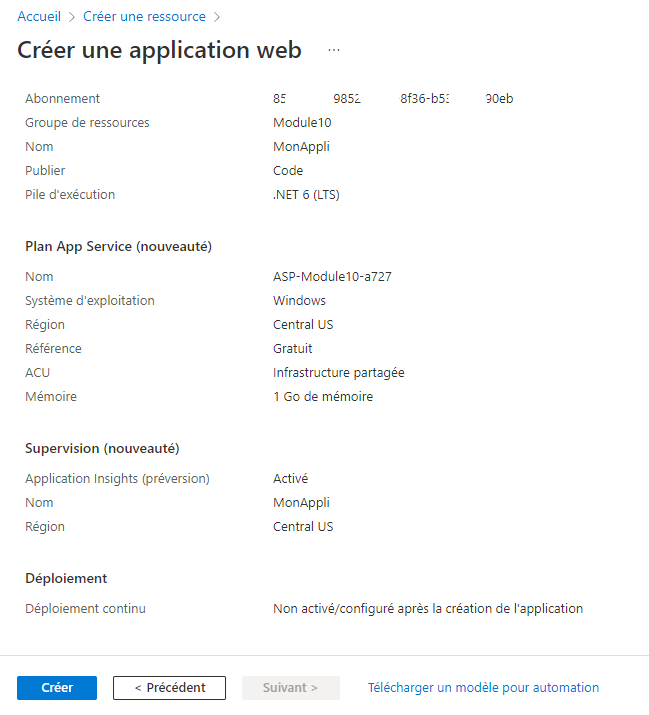
\includegraphics[scale=0.5]{images/capture1}
			
		\end{figure}
		\item Maintenant il faut décompacter : \index{tar}
		\begin{lstlisting}[language=bash]   ]
		$sudo tar xvf openjdk-11.0.2_linux-x64_bin.tar.gz --directory /usr/lib/jvm/
		\end{lstlisting}
		\item et installer le java et le javac (compilateur)\index{update-alternatives}
		\begin{lstlisting}[language=bash]   ]
		$sudo update-alternatives --install /usr/bin/java java /usr/lib/jvm/jdk-11.0.2/bin/java 1
		\end{lstlisting}
		
		\begin{lstlisting}[language=bash]   ]
		$sudo update-alternatives --install /usr/bin/javac javac /usr/lib/jvm/jdk-11.0.2/bin/javac 1
		\end{lstlisting}
		
		\begin{figure}[!htb]
			\centering
			\includegraphics[scale=0.65]{images/capture2}
		\end{figure}
\subsubsection{Création d'un application Java}
		
		\item Vérifion le fonctionnement de Java en créant notre votre premier programme dans un éditeur de texte(gedit ou autre éditeur):  \index{gedit}
		\begin{lstlisting}[language=bash]   ]
		$gedit helloWorld.java
		\end{lstlisting}
		\item sassiez le code suivant :
		\textbf{Syntaxe}
		\begin{lstlisting}[
		language=SQL,
		showspaces=false,
		basicstyle=\scriptsize,
		captionpos=b, 
		frame=single,   
		showstringspaces=false,
		commentstyle=\color{mongris},
		backgroundcolor=\color{backcolour},
		keywordstyle=\color{blue},   
		numberstyle=\tiny\color{mongris}, 
		rulecolor=\color{black}, 
		stringstyle=\color{red},
		]
		class helloWorld {
		
		public static void main(String args[]){
		System.out.println("Bonjour tout le monde!");
		}
		}
		
		\end{lstlisting}
		
		\item Puis dans le terminal, dans le répertoire où se trouve votre fichier helloWord.java: 
		
		\index{javac}
		\begin{lstlisting}[language=bash]   ]
		$javac helloWorld.java
		\end{lstlisting}
		ce qui compile votre code et crée le fichier helloWorld.class.\\
		On peut maintenant lancée l'exécution: \index{java}
		\begin{lstlisting}[language=bash]   ]
		$java helloWorld
		\end{lstlisting}
		\begin{figure}[!htb]
			\centering
			\includegraphics[scale=0.99]{images/capture3}
			
		\end{figure}
		
	\end{itemize}
	\subsection{Installer .NET Core }
	
	Nous allons utiliser le gestionnaire de packet pour installer .NET Core sur Ubuntu comme le décrit Microsoft dans son article\footnote{Source  : \url{https://docs.microsoft.com/en-us/dotnet/core/install/linux-package-manager-ubuntu-2004}}.
	
	\subsubsection{Installation de .NET Core SDK}
	Avant d'installer .NET, vous devrez:
	\begin{itemize}
		\item Ajoutez la clé de signature du package Microsoft à la liste des clés approuvées.
		\item Ajoutez le référentiel au gestionnaire de packages.
		\item Installez les dépendances requises.
		
		Ouvrez un terminal et exécutez les commandes suivantes:\index{wget} \index{dpkg}
		\begin{lstlisting}[language=bash]   ]
		$wget https://packages.microsoft.com/config/ubuntu/20.04/packages-microsoft-prod.deb -O packages-microsoft-prod.deb
		$sudo dpkg -i packages-microsoft-prod.deb
		\end{lstlisting}
		
		Mettez à jour les produits disponibles pour l'installation, puis installez le SDK .NET Core. Dans votre terminal, exécutez les commandes suivantes:\index{apt-get!update}\index{apt-get!upgrade}\index{apt-get!install}
		\begin{lstlisting}[language=bash]   ]
		$sudo apt-get update
		$sudo apt-get install apt-transport-https
		$sudo apt-get update
		$sudo apt-get install dotnet-sdk-3.1
		\end{lstlisting}
		
		Vérifier votre installation en tapant la commande suivante \index{dotnet!--info}
		
		\begin{lstlisting}[language=bash]   ]
		$dotnet --info
		\end{lstlisting}
		
		
	\end{itemize}
	
	
	\subsubsection{Création d'une application C \#}
	Tapez les commandes dotnet suivantes pour créer et exécuter une application C \#:
	\index{dotnet!new}\index{dotnet!run}
	\begin{lstlisting}[language=bash]   ]
	$dotnet new console --output sample1
	$dotnet run --project sample1
	\end{lstlisting}
	
	Vous devriez voir la sortie suivante:
	
	\begin{figure}[!htb]
		\centering
		\includegraphics[scale=0.8]{images/capture4}
		
	\end{figure}
	
	
	\subsection{Système de gestion de base de données}
	Au niveau SGBD, une diversité de produit s'offre à nous. Au niveau relationnel :  Oracle, SQL Serveur de  Micrososft, PostgreSQL. Au niveau NoSQL : MongoDB, Redis, HBase, Cassandra et bien d'autres.
	
	
	\textbf{Nous allons opter pour celui qui est généralement utilisé avec dans le développement de site Web avec PHP, MySQL.}
	
	\subsubsection{Installation MySQL Serveur 8.0}
	
	\begin{itemize}
		\item  Vérifion ce que le gestionnaire de paquet (APT) nous offre avec la commande :\index{apt!cache}
		\begin{lstlisting}[language=bash]   ]
		$sudo apt update
		$sudo apt-cache search mysql-server
		\end{lstlisting}
		
		\item Voici ma sortie :
		\begin{figure}[!htb]
			\centering
			\includegraphics[scale=0.5]{images/capture5}
		\end{figure}
		
		\item Nous allons utiliser la version mysql-server-8.0
		\begin{lstlisting}[language=bash]   ]
		$sudo apt install mysql-server-8.0
		\end{lstlisting}
		
		\begin{figure}[!htb]
			\centering
			\includegraphics[scale=0.5]{images/capture6}
		\end{figure}
		
		\item Répondez {\color{blue}oui}
		
		\item Par défaut, MySQL manque de nombreuses fonctionnalités de sécurité de base et importantes. Heureusement, il est livré avec un script d'installation qui vous guide à travers la configuration.
		
		\item Pour installer le script de sécurité MySQL, entrez:  \begin{lstlisting}[language=bash]   ]
		$sudo mysql_secure_installation
		\end{lstlisting}
		\begin{figure}[!htb]
			\centering
			\includegraphics[scale=0.7]{images/capture7}
		\end{figure}
		
		\item Le système vous demandera le mot de passe root MySQL. Tapez {\color{blue}Y}
		\item Ensuite, le programme d'installation décrira les fonctionnalités du plugin Validate Password. Vous devrez sélectionner le niveau de sécurité. Je vous recommande {\color{blue}0 pour LOW }. Nous ne sommes pas en production, mais en développement. Donc le niveau de sécurité et un peu moins importants.
		
		
		\begin{figure}[!htb]
			\centering
			\includegraphics[scale=0.7]{images/capture8}
		\end{figure}
		
		\item Changer le mot de passe root : \\
		Ensuite, le programme d'installation vous offrira la possibilité de changer le mot de passe pour root. Tapez y pour modifier le mot de passe.
		
		\item Si vous modifiez le mot de passe, il devra suivre toutes les exigences que vous avez configurées à l'étape précédente.
		
		\item Le système vous demandera les fonctions de sécurité suivantes. Il est recommandé de confirmer (tapez y) toutes les options, sauf si vous avez une raison de les garder désactivées.
		\begin{itemize}
			\item Supprimer les utilisateurs anonymes? {\color{blue}Y}
			\item Désactiver la connexion root à distance? {\color{blue}Y}
			\item Supprimer la base de données de test et y accéder? {\color{blue}Y}
			\item Recharger les tables de privilèges maintenant? {\color{blue}Y}
			
		\end{itemize}
		
		\textbf{Démarrer, arrêter ou vérifier l'état du service MySQL}\\
		Dans Ubuntu, le service MySQL devrait démarrer automatiquement.\\
		
		\begin{itemize}
			\item  Pour vérifier que MySQL fonctionne, entrez la commande:\index{service}
			
			
			\begin{lstlisting}[language=bash]   ]
			$sudo service mysql status
			\end{lstlisting}
		\end{itemize}
		
		\begin{figure}[!htb]
			\centering
			\includegraphics[scale=0.7]{images/capture9}
		\end{figure} 
		\item Pour arrêter, démarrer ou redémarrer MySQL : 
		\begin{lstlisting}[language=bash]   ]
		$sudo service mysql stop
		$sudo service mysql start
		ou
		$sudo service mysql restart
		\end{lstlisting}
		\item Nous allons maintenant vérifier les connexions possibles au serveur MySQL :
		\item, Mais avant nous devons installer les outils {\color{blue}net-tools}\index{netstat}
		\begin{lstlisting}[language=bash]   ]
		$sudo apt install net-tools
		$netstat -paunt |grep 3306
		\end{lstlisting}
		
		\begin{figure}[!htb]
			\centering
			\includegraphics[scale=0.7]{images/capture11}
		\end{figure} 
	 MySQL écoute sur les ports (TCP 3306 et tcp6 33060). La cinquième colonne représente les adresses distantes. Donc MySQL accepte les connexions distantes, peu importe l'origine. Mais ce n'est pas ici qu'on voit que  root est bloqué sauf en localhost. C'est dans un fichier de configuration de MySQL.
	\end{itemize}
	
	\subsubsection{Tester l'installation de MySQL}
	
	Le client MySQL a également été installé. Nous allons l'utiliser pour tester notre installation.
	
	\begin{itemize}
		\item Tapez la commande suivante pour accéderr au client : 

	\begin{lstlisting}[language=bash]   ]
	$sudo mysql -u root -p
	\end{lstlisting}
	
	Vous pouvez maintenant tester vos requêtes SQL.
	\begin{lstlisting}[language=bash]   ]
	mysql>show databases
	\end{lstlisting}
	
	\begin{figure}[!htb]
		\centering
		\includegraphics[scale=0.45]{images/capture12}

	\end{figure}

	\item Nous allons créer un administrateur de base de données pouvant se connecter à distance :
	
	\begin{lstlisting}[language=bash]   ]
	mysql >CREATE USER 'admindb'@'%' identified bye 'LeMotDePasse';
	\end{lstlisting}
	\item Pour accorder à l’utilisateur tous les privilèges pour la base de données et la possibilité de les transmettre, exécutez la commande suivante:
	\begin{lstlisting}[language=bash]   ]
	mysql >GRANT ALL PRIVILEGES ON *.* TO 'admindb'@'%' WITH GRANT OPTION;
	\end{lstlisting}
	\item Pour que les changements prennent effet, appliquez immédiatement les privilèges en tapant la commande suivante:
	\begin{lstlisting}[language=bash]   ]
	mysql>FLUSH PRIVILEGES;
	\end{lstlisting}
	\item Tapez {\color{blue}exit} pour sortir du client.
	\item Connectez-vous avec votre nouvel usager pour vérifier ses droits.
	
	
	\begin{figure}[!htb]
		\centering
		\includegraphics[scale=0.8]{images/capture14}
	\end{figure}
	
	\end{itemize}  
	
%	\subsubsection{Installer MySQL Workbench}
%	À l'aide de l'outil Ubuntu Software installer MySQL Workbench :
%	\begin{figure}[!htb]
%		\centering
%		\includegraphics[scale=0.5]{images/capture10}
%	\end{figure}
%	
	
	\section{Enrionnement de développement}
	\subsection{IDE : Eclipse}
	Eclipse est un IDE (environnement de développement intégré) écrit en Java, extensible par des greffons, multi-langages et multi-plates-formes, qui s'intègre particulièrement bien à GNOME.
	
	Il est d'abord conçu pour le langage Java, mais ses nombreux greffons en font un environnement de développement pour de nombreux autres langages de programmation (C/C++, Python, PHP, Ruby, …).
	
	Toutes les fonctions qu'on peut attendre de ce genre de logiciel sont présentes ou existent sous forme de greffons (coloration syntaxique, complétion, debugger, gestion de projets, intégration aux gestionnaires de versions, …). \footnote{Source : https://doc.ubuntu-fr.org/eclipse}
	
	
	\begin{itemize}
		\item  Eclipse Installer est téléchargeable à l'adresse suivante \url{https://eclipse.org/downloads/}, ou bien ici : \url{https://wiki.eclipse.org/Eclipse\_Installer}. Il se présente sous la forme d'une archive tar.gz (exemple : eclipse-inst-linux64.tar.gz) à décompresser dans le répertoire permanent de votre choix (par défaut : eclipse-installer) dans votre 'HOME'. 
	\index{tar}\index{cd}\index{./}
	\begin{lstlisting}[language=bash]   
	$tar xvfz  ~/Téléchargements/eclipse-inst-linux64.tar.gz
	$cd eclipse-installer
	$./eclipse-inst
	\end{lstlisting}
	\item Sélectionnez Eclipse IDE for java Developper. 
	
	
	\item Suivre les instructions en cliquant sur {\color{orange}Install} situé en bas dans la seconde fenêtre en faisant bien attention de retenir les répertoires que l'outil va créer sous votre répertoire \$HOME/eclipse. 
\end{itemize}
	\subsection{Visual Studio Code}
	
	Allez sur cette page \url{https://code.visualstudio.com/download}, et sélectionnez le fichier "deb (Debian, Ubuntu)" en 64. Installez-le en ligne de commande :
	\begin{itemize}
		\item Taper les commandes suivantes :
		
		\begin{lstlisting}[language=bash]  
		$cd Téléchargements
		$sudo dpkg -i code_*.deb
		\end{lstlisting}
		
		\item Maintenant allez dans Afficher les applications en bas à gauche, taper visual...et vous le voyez apparaitre.
		
		\item Lancer le.
		\item Vous pouvez aussi en profiter pour mettre un favori en cliquant  avec votre souris sur le bonton droit dans la barre de gauche et l'ajouter aux favoris.
		
		
		
		
		\begin{figure}[!htb]
			\centering
			\includegraphics[scale=0.8]{images/capture13}
		\end{figure}
		\item Bien sur, vous pouvez en profiter pour ajouter les applications régulièrement utilisées.


		
	\end{itemize}
	
\section{Espace disque après installation}
Vérifier maintenant l'espace disque utilisé après les installations.
\index{df}
\begin{lstlisting}[language=bash]   ]
$df -h |grep /dev/sda > Bureau/espaceDiskAprestInstallation.txt
\end{lstlisting}

Le fichier étant maintenant su le bureau, vous voir après l'espace qui à été utilisé par nos installations.

Comparrer le fichier avant celui produit avant l'installation.
	
	\vspace{2cm}
	\textbf{ Fin de l'exercice \exercice.}
	
	
	
	
	
	
	
	\section{Compétences développées en partie dans l'exercice \exercice}
	\begin{tabular}{|p{5cm}|l|}
		\hline
		\textbf{Énoncé(s) de compétence}&\textbf{Élément de la compétence} \\[3pt]
		\hline
		00Q1 - Effectuer l’installation et la gestion d’ordinateur&2 installer le système d’exploitation.\\
		&3 Installer des applications\\
		&4 Effectuer des tâches de gestion du système d’exploitation.\\
		\hline
		00SF - Évaluer des composants logiciels et
		matériels&1 Rechercher des composants logiciels et matériels.\\
		&2 Formuler des avis sur les composants logiciels et matériels.\\
		\hline
		
	\end{tabular}
	
	
	\printindex
	
	
	
	\renewcommand{\contentsname}{Sommaire} % Dans le corps du document,avant la commande \tableofcontents.
	
	\setcounter{tocdepth}{5}
	
	\addcontentsline{toc}{section}{Sommaire}
	
	\tableofcontents
	
	\pagebreak
	
	
	\addcontentsline{toc}{section}{Références}
	
	\nocite{*}
	
	
	
	\textbf{Cette liste de références contient également des lectures suggérées pour approfondir le sujet.}\\
	\printbibliography
	
	
	\rule{\linewidth}{1pt}\\
	
	\textbf{\textit{Ce document a été écrit avec LaTeX}.}\\
	
	%\includegraphics[scale=1]{88x31.png}\\
	
	\shadowbox{\parbox{15cm}
		{Cette oeuvre, création, site ou texte est sous licence Creative Commons Attribution - Pas d’Utilisation commerciale - Partage dans les Mêmes Conditions 4.0 International. Pour accéder à une copie de cette licence, merci de vous rendre à l'adresse suivante \url{http://creativecommons.org/licenses/by-nc-sa/4.0/} \\ ou envoyez un courrier à Creative Commons, 444 Castro Street, Suite 900, Mountain View, California, 94041, USA.}}
	
\end{document}

